\documentclass{article}
\usepackage{graphicx}
\usepackage{float}
\usepackage{fullpage}

\begin{document}

\begin{tabular}{rl}
  \textbf{Lab 9:} & Three Phase Induction Motor\\
  \textbf{Performed:} & April 01, 2013 \\
  \textbf{Partners:} & Rawley Dent \\ & Charles Pittman \\
  \textbf{Instructor:} & Dr.\ Weatherford
\end{tabular}


\section*{Abstract}
  In this experiment, the basic principles of an induction motor were studied.
  Using a wound-rotor motor at two different supply voltages, the motor's
  speed, torque output, and line current was recording at various load torques.

\section*{Results}
  \begin{figure}[H]
    \centering
    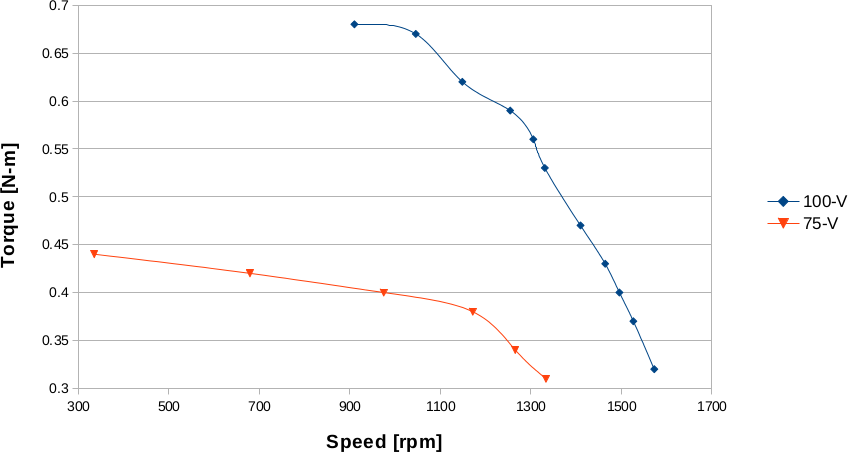
\includegraphics[width=\textwidth]{img/graph}
    \caption{\textbf{Comparison of Output Torque vs. Speed for Different Supply Voltages}}
    \label{fig:graph}
  \end{figure}

\section*{Conclusions}
  In a typical torque speed curve, the plot rises sharply from the starting
  torque to the breakdown (peak) torque, and then decreases linearly to the
  no-load mark. This linear section is the motor's operating region.

  As shown in Fig~\ref{fig:graph} the no-load torque is not changed, but occurs
  at a slower speed with a reduced starting voltage.  Since the rotor acts as
  though there is no load, this is also the synchronous speed, so lowering the
  starting voltage also reduces synchronous speed.  The torque developed is
  proportional to the square of supplied voltage, thus a relatively small
  reduction in supplied voltage here drastically changes the the operating
  region.  The higher starting voltage has much higher starting and breakdown
  torques.

\end{document}
